\documentclass[10pt]{article}
%DIF LATEXDIFF DIFFERENCE FILE
%DIF DEL kindle_v6.tex          Sat Nov 21 19:43:12 2026
%DIF ADD exact_raf_kindle.tex   Sat Nov 21 20:16:44 2026
\usepackage[paperwidth=100mm,paperheight=135mm,left=4mm,right=4mm,top=5mm,bottom=7mm,footskip=4mm]{geometry}
\usepackage{float}
\usepackage{adjustbox}
\sloppy
\setlength{\emergencystretch}{3em}
\usepackage[T1]{fontenc}
\usepackage{mathptmx}
\usepackage{amsmath,amssymb,amsthm}
\usepackage{booktabs}
\usepackage{graphicx}
\usepackage{url}
\usepackage{algorithm}
\usepackage{algpseudocode}

\newtheorem{theorem}{Theorem}
\newtheorem{propo}{Proposition}
\newtheorem{lemma}{Lemma}
\newtheorem{corollary}{Corollary}
\theoremstyle{definition}
\newtheorem{example}{Example}
\newtheorem{remark}{Remark}

\newcommand{\U}{\mathbf{U}}
\newcommand{\R}{\mathbb{R}}
\newcommand{\eps}{\varepsilon}
\newcommand{\ex}{\eps_x}
\newcommand{\ey}{\eps_y}
\newcommand{\rng}{\operatorname{rng}}
\newcommand{\wid}{\operatorname{wid}}
\newcommand{\mmid}{\operatorname{mid}}

\title{Exact multiplication of reduced affine forms}
\author{Ignacio Araya \and Daniel Miranda \and Victor Reyes \and Juan Geraldo}
\date{\small Kindle version \DIFdelbegin \DIFdel{v6 }\DIFdelend \DIFaddbegin \DIFadd{v7 }\DIFaddend (2026-11-21)}

\usepackage{fancyhdr}
%DIF 37c37
%DIF < \fancypagestyle{plain}{\fancyhf{}\renewcommand{\headrulewidth}{0pt}\cfoot{\thepage}\rfoot{\tiny v6}}
%DIF -------
\fancypagestyle{plain}{\fancyhf{}\renewcommand{\headrulewidth}{0pt}\cfoot{\thepage}\rfoot{\tiny v7}} %DIF > 
%DIF -------
\pagestyle{plain}
%DIF PREAMBLE EXTENSION ADDED BY LATEXDIFF
%DIF CFONT PREAMBLE %DIF PREAMBLE
\RequirePackage{color}\definecolor{RED}{rgb}{1,0,0}\definecolor{BLUE}{rgb}{0,0,1} %DIF PREAMBLE
\DeclareOldFontCommand{\sf}{\normalfont\sffamily}{\mathsf} %DIF PREAMBLE
\providecommand{\DIFadd}[1]{\highLight[hlgray]{#1}} %DIF PREAMBLE
\providecommand{\DIFdel}[1]{{\protect\color{red}\strikeThrough{#1}}} %DIF PREAMBLE
%DIF SAFE PREAMBLE %DIF PREAMBLE
\providecommand{\DIFaddbegin}{} %DIF PREAMBLE
\providecommand{\DIFaddend}{} %DIF PREAMBLE
\providecommand{\DIFdelbegin}{} %DIF PREAMBLE
\providecommand{\DIFdelend}{} %DIF PREAMBLE
\providecommand{\DIFmodbegin}{} %DIF PREAMBLE
\providecommand{\DIFmodend}{} %DIF PREAMBLE
%DIF FLOATSAFE PREAMBLE %DIF PREAMBLE
\providecommand{\DIFaddFL}[1]{\DIFadd{#1}} %DIF PREAMBLE
\providecommand{\DIFdelFL}[1]{\DIFdel{#1}} %DIF PREAMBLE
\providecommand{\DIFaddbeginFL}{} %DIF PREAMBLE
\providecommand{\DIFaddendFL}{} %DIF PREAMBLE
\providecommand{\DIFdelbeginFL}{} %DIF PREAMBLE
\providecommand{\DIFdelendFL}{} %DIF PREAMBLE
\newcommand{\DIFscaledelfig}{0.5}
%DIF HIGHLIGHTGRAPHICS PREAMBLE %DIF PREAMBLE
\RequirePackage{settobox} %DIF PREAMBLE
\RequirePackage{letltxmacro} %DIF PREAMBLE
\newsavebox{\DIFdelgraphicsbox} %DIF PREAMBLE
\newlength{\DIFdelgraphicswidth} %DIF PREAMBLE
\newlength{\DIFdelgraphicsheight} %DIF PREAMBLE
% store original definition of \includegraphics %DIF PREAMBLE
\LetLtxMacro{\DIFOincludegraphics}{\includegraphics} %DIF PREAMBLE
\newcommand{\DIFaddincludegraphics}[2][]{{\color{blue}\fbox{\DIFOincludegraphics[#1]{#2}}}} %DIF PREAMBLE
\newcommand{\DIFdelincludegraphics}[2][]{% %DIF PREAMBLE
\sbox{\DIFdelgraphicsbox}{\DIFOincludegraphics[#1]{#2}}% %DIF PREAMBLE
\settoboxwidth{\DIFdelgraphicswidth}{\DIFdelgraphicsbox} %DIF PREAMBLE
\settoboxtotalheight{\DIFdelgraphicsheight}{\DIFdelgraphicsbox} %DIF PREAMBLE
\scalebox{\DIFscaledelfig}{% %DIF PREAMBLE
\parbox[b]{\DIFdelgraphicswidth}{\usebox{\DIFdelgraphicsbox}\\[-\baselineskip] \rule{\DIFdelgraphicswidth}{0em}}\llap{\resizebox{\DIFdelgraphicswidth}{\DIFdelgraphicsheight}{% %DIF PREAMBLE
\setlength{\unitlength}{\DIFdelgraphicswidth}% %DIF PREAMBLE
\begin{picture}(1,1)% %DIF PREAMBLE
\thicklines\linethickness{2pt} %DIF PREAMBLE
{\color[rgb]{1,0,0}\put(0,0){\framebox(1,1){}}}% %DIF PREAMBLE
{\color[rgb]{1,0,0}\put(0,0){\line( 1,1){1}}}% %DIF PREAMBLE
{\color[rgb]{1,0,0}\put(0,1){\line(1,-1){1}}}% %DIF PREAMBLE
\end{picture}% %DIF PREAMBLE
}\hspace*{3pt}}} %DIF PREAMBLE
} %DIF PREAMBLE
\LetLtxMacro{\DIFOaddbegin}{\DIFaddbegin} %DIF PREAMBLE
\LetLtxMacro{\DIFOaddend}{\DIFaddend} %DIF PREAMBLE
\LetLtxMacro{\DIFOdelbegin}{\DIFdelbegin} %DIF PREAMBLE
\LetLtxMacro{\DIFOdelend}{\DIFdelend} %DIF PREAMBLE
\DeclareRobustCommand{\DIFaddbegin}{\DIFOaddbegin \let\includegraphics\DIFaddincludegraphics} %DIF PREAMBLE
\DeclareRobustCommand{\DIFaddend}{\DIFOaddend \let\includegraphics\DIFOincludegraphics} %DIF PREAMBLE
\DeclareRobustCommand{\DIFdelbegin}{\DIFOdelbegin \let\includegraphics\DIFdelincludegraphics} %DIF PREAMBLE
\DeclareRobustCommand{\DIFdelend}{\DIFOaddend \let\includegraphics\DIFOincludegraphics} %DIF PREAMBLE
\LetLtxMacro{\DIFOaddbeginFL}{\DIFaddbeginFL} %DIF PREAMBLE
\LetLtxMacro{\DIFOaddendFL}{\DIFaddendFL} %DIF PREAMBLE
\LetLtxMacro{\DIFOdelbeginFL}{\DIFdelbeginFL} %DIF PREAMBLE
\LetLtxMacro{\DIFOdelendFL}{\DIFdelendFL} %DIF PREAMBLE
\DeclareRobustCommand{\DIFaddbeginFL}{\DIFOaddbeginFL \let\includegraphics\DIFaddincludegraphics} %DIF PREAMBLE
\DeclareRobustCommand{\DIFaddendFL}{\DIFOaddendFL \let\includegraphics\DIFOincludegraphics} %DIF PREAMBLE
\DeclareRobustCommand{\DIFdelbeginFL}{\DIFOdelbeginFL \let\includegraphics\DIFdelincludegraphics} %DIF PREAMBLE
\DeclareRobustCommand{\DIFdelendFL}{\DIFOaddendFL \let\includegraphics\DIFOincludegraphics} %DIF PREAMBLE
%DIF COLORLISTINGS PREAMBLE %DIF PREAMBLE
\RequirePackage{listings} %DIF PREAMBLE
\RequirePackage{color} %DIF PREAMBLE
\lstdefinelanguage{DIFcode}{ %DIF PREAMBLE
%DIF DIFCODE_CFONT %DIF PREAMBLE
  moredelim=[il][\color{red}\scriptsize]{\%DIF\ <\ }, %DIF PREAMBLE
  moredelim=[il][\color{blue}\sffamily]{\%DIF\ >\ } %DIF PREAMBLE
} %DIF PREAMBLE
\lstdefinestyle{DIFverbatimstyle}{ %DIF PREAMBLE
	language=DIFcode, %DIF PREAMBLE
	basicstyle=\ttfamily, %DIF PREAMBLE
	columns=fullflexible, %DIF PREAMBLE
	keepspaces=true %DIF PREAMBLE
} %DIF PREAMBLE
\lstnewenvironment{DIFverbatim}{\lstset{style=DIFverbatimstyle}}{} %DIF PREAMBLE
\lstnewenvironment{DIFverbatim*}{\lstset{style=DIFverbatimstyle,showspaces=true}}{} %DIF PREAMBLE
%DIF END PREAMBLE EXTENSION ADDED BY LATEXDIFF

\usepackage{luacolor}
\usepackage{lua-ul}
\definecolor{hlgray}{gray}{0.78}
\begin{document}
\maketitle

\begin{abstract}
Reduced affine forms keep a fixed number of noise symbols and accumulate all the approximation errors in a single error term. The product of two such forms must be enclosed by a new reduced affine form, and the width of this enclosure determines the quality of range bounds and of the linear relaxations built from the forms in branch-and-bound solvers. Skalna and Hlad\'{\i}k computed in linear time the exact range of the quadratic part of the product. We show that their multiplication is not exact when both operands carry errors, because the terms that couple the centers of the operands with their error symbols are bounded separately, and we give a multiplication that computes the exact range of the whole nonlinear part of the product in $O(n\log n)$ time, by four walks along the boundary of a planar zonotope. We prove that it coincides with that of Skalna and Hlad\'{\i}k when one operand has no error or a zero center, and that it is at most $3/2$ times narrower otherwise, a tight bound. We also give a rigorous floating-point implementation of both multiplications. In an interval branch-and-bound optimizer, replacing the standard multiplication used by default by either of them reduces the number of nodes about four times on problems dominated by products; the new multiplication saves a further 4--7\% of the nodes exactly on the problems where the theory predicts a gain, and coincides with that of Skalna and Hlad\'{\i}k elsewhere.

\medskip\noindent
\textit{Keywords:} reduced affine arithmetic, multiplication, range enclosure, linear relaxation, zonotope
\end{abstract}

\section{Introduction}

Affine arithmetic (AA)~\cite{combastolfi1993,stolfi1997self,defigueiredo2004affine} represents an uncertain quantity by an affine function of noise symbols $\eps_i\in\U=[-1,1]$, and keeps the linear dependencies between quantities that share symbols. Each nonlinear operation of standard AA introduces a new symbol, so the forms grow along long computations. Reduced affine forms~\cite{messine2002extentions,vu2009enhancing,skalna2017new} keep only the $n$ symbols of the initial uncertain parameters and accumulate all the errors in one term,
\begin{equation}
\label{eq:raf}
\hat x = x_0 + \sum_{i=1}^n x_i\eps_i + x_r\ex,\qquad x_r\ge 0,\ \ex\in\U .
\end{equation}
They are the basis of the reliable affine relaxations used in interval branch-and-bound solvers~\cite{ninin2015reliable}: over a box, each $\eps_i$ is an affine function of the variable $x_i$, so that a form is a linear function of the variables plus an interval, and its two bounding hyperplanes are a range enclosure and a linear relaxation of the corresponding expression. The vertical distance between them, $2x_r$, measures the quality of the relaxation.

The product of two reduced affine forms is a quadratic function of the symbols and must be enclosed by a new reduced affine form. The multiplications proposed in the literature keep the same linear part and differ in how they enclose the remaining nonlinear terms, which consist of the quadratic part $(e^Tx+x_r\ex)(e^Ty+y_r\ey)$ and of the terms $x_0y_r\ey+y_0x_r\ex$ that couple the center of each operand with the error of the other (Section~\ref{sec:products}):
\begin{itemize}
\item The \emph{trivial} multiplication of standard AA~\cite{stolfi1997self} bounds the quadratic part by the product of the total radii of the operands, $(\|x\|_1+x_r)(\|y\|_1+y_r)$, as if all its terms could reach their largest absolute values at the same time.
\item The \emph{standard} multiplication~\cite{kolev2004improved,vu2009enhancing} uses that the squares $\eps_i^2$ range over $[0,1]$ instead of $[-1,1]$: it moves the center by $\tfrac12x^Ty$ and removes $\tfrac12|x|^T|y|$ from the radius. AF2~\cite{messine2002extentions} exploits the same fact differently, by keeping two one-sided error terms for the positive and the negative squares.
\item A formula attributed to Miyajima~\cite{skalna2017new} also groups the two bilinear terms $x_iy_j\eps_i\eps_j$ and $x_jy_i\eps_j\eps_i$ of each pair before bounding them, which helps when they cancel.
\item The \emph{best multiplication} of Miyajima, Miyata and Kashiwagi~\cite{miyajima2003best}, implemented in the kv library~\cite{kvlib}, computes the exact range of the whole quadratic part, including the error symbols of the operands, in $O(n^2)$ time.
\item Skalna and Hlad\'{\i}k~\cite{skalna2017new} compute the same exact range in linear time. They observe that $(e^Tx,e^Ty)$ ranges over a planar zonotope, whose boundary is described by the generators $(x_i,y_i)$ sorted by angle, and that the product $uv$ attains its extrema on that boundary. They describe their multiplication as yielding the minimum Chebyshev-type bounds, and it is the tightest of the existing formulae.
\end{itemize}
The exact methods stop at the quadratic part because in standard AA it is all that has to be bounded: the terms $x_0(\hat y-y_0)+y_0(\hat x-x_0)$ stay as linear terms in their own symbols, and Rump and Kashiwagi~\cite{rump2015implementation} refer to~\cite{miyajima2003best} for the optimal bound of the quadratic part. In reduced affine forms, however, the terms $x_0y_r\ey+y_0x_r\ex$ involve the error symbols of the operands and must be folded into the new error term, and both the kv implementation for forms with an accumulated error term and the multiplication of Skalna and Hlad\'{\i}k add their bound $|y_0|x_r+|x_0|y_r$ separately.

In this paper we observe that the multiplication of Skalna and Hlad\'{\i}k is not exact when both operands carry errors: two terms of the product, $x_0 y_r\ey$ and $y_0 x_r\ex$, are bounded separately from the quadratic part, although they share the error symbols with it. We show that the whole nonlinear part of the product is affine in each of the two error symbols, so that its range is the union of four ranges obtained with the error symbols fixed at the vertices of $\U^2$; for each vertex, what remains is a product of two shifted linear functions of the symbols, whose exact range follows from the geometry of planar zonotopes used by Skalna and Hlad\'{\i}k. The resulting multiplication computes the exact range of the nonlinear part of the product, in $O(n\log n)$ time.

\paragraph{Contributions.}
\begin{itemize}
\item An exact multiplication of reduced affine forms, E (Section~\ref{sec:exact}): Theorem~\ref{thm:exact} shows that it gives the narrowest enclosure of the product with the usual linear part, and Algorithm~\ref{alg:exact} computes it in $O(n\log n)$ time.
\item Its relation with the existing formulae (Section~\ref{sec:hierarchy}): E is contained in the multiplication SH of Skalna and Hlad\'{\i}k, which is contained in the standard and trivial ones; E coincides with SH when one operand has no error (Proposition~\ref{prop:oneerror}) and is at most $3/2$ times narrower otherwise, a tight bound (Proposition~\ref{prop:32}); the difference of widths is at most $2\min(|x_0|y_r,|y_0|x_r)$, and usually equal to it, so that E can only help when both operands carry errors and have nonzero centers (Corollary~\ref{cor:gain}). We also show that the standard multiplication is AF2~\cite{messine2002extentions} with its one-sided error terms re-centered after each product (Proposition~\ref{prop:af2}).
\item A rigorous floating-point implementation of SH and E (Section~\ref{sec:rigor}), with an exact angular predicate and an a priori bound of the rounding errors of the boundary walk.
\item Experiments (Section~\ref{sec:experiments}) on range enclosures, with exact ranges computed by a global optimizer, and in an interval global optimizer, where the exact-range multiplications reduce the search tree about four times on problems dominated by products, and E improves on SH exactly where Corollary~\ref{cor:gain} predicts.
\end{itemize}

\section{Products of reduced affine forms}
\label{sec:products}

Let $\hat x$ be as in~\eqref{eq:raf} and $\hat y = y_0+\sum_i y_i\eps_i + y_r\ey$, and write $x=(x_1,\dots,x_n)$, $y=(y_1,\dots,y_n)$ and $e=(\eps_1,\dots,\eps_n)\in\U^n$. Following~\cite{skalna2017new},
\begin{equation}
\label{eq:product}
\hat x\hat y = x_0y_0 + e^T(y_0x+x_0y) + N(e,\ex,\ey),
\end{equation}
\begin{equation}
\label{eq:N}
N(e,\ex,\ey) = x_0y_r\ey + y_0x_r\ex + (e^Tx + x_r\ex)(e^Ty + y_r\ey).
\end{equation}
All the formulae considered here keep the linear part $x_0y_0+e^T(y_0x+x_0y)$ and enclose $N$ over $\U^{n+2}$ by an interval $[c-z_r,\,c+z_r]$, which gives the reduced affine form
\begin{equation}
\label{eq:zhat}
\hat z = x_0y_0 + c + e^T(y_0x+x_0y) + z_r\eps_z .
\end{equation}
A multiplication formula is therefore an enclosure of $\rng N$, the range of $N$ over $\U^{n+2}$, and its quality is the width $2z_r$, the thickness of the resulting relaxation. Denote $\|x\|_1=\sum_i|x_i|$, $|x|=(|x_1|,\dots,|x_n|)$, and
\[
\begin{gathered}R(e,\ex,\ey) = (e^Tx + x_r\ex)(e^Ty + y_r\ey),\\ Q(e) = (e^Tx)(e^Ty) = \sum_i x_iy_i\eps_i^2 + \sum_{i<j}(x_iy_j+x_jy_i)\eps_i\eps_j .\end{gathered}
\]
We consider the following formulae, labeled as in~\cite{skalna2017new} when they appear there.
\begin{description}
\item[T, trivial~\cite{stolfi1997self} (Eq.~4 of~\cite{skalna2017new}).] $c=0$, $z_r = |y_0|x_r+|x_0|y_r+(\|x\|_1+x_r)(\|y\|_1+y_r)$.
\item[S, standard~\cite{kolev2004improved,vu2009enhancing} (Eq.~5).] $c=\tfrac12 x^Ty$, $z_r = |y_0|x_r+|x_0|y_r+(\|x\|_1+x_r)(\|y\|_1+y_r) - \tfrac12|x|^T|y|$. The squares $x_iy_i\eps_i^2\in x_iy_i[0,1]$ are enclosed by their exact range.
\item[SH, Skalna and Hlad\'{\i}k~\cite{skalna2017new} (Eq.~10).] $[c-z_r,c+z_r] = [R_{\min},R_{\max}] + [-1,1](|y_0|x_r+|x_0|y_r)$, where $[R_{\min},R_{\max}]=\rng R$ is computed exactly in $O(n)$ time. The best multiplication of~\cite{miyajima2003best}, as implemented in the kv library~\cite{kvlib} (option \texttt{AFFINE\_MULT=2}), gives the same interval, with an $O(n^2)$ algorithm.
\item[E, exact (this paper).] $[c-z_r,c+z_r]=\rng N$.
\end{description}
Skalna and Hlad\'{\i}k also consider an intermediate formula attributed to Miyajima (Eq.~6 of~\cite{skalna2017new}), which groups the two bilinear terms $x_iy_j$ and $x_jy_i$ of each pair before bounding them; it lies between SH and S~\cite[Prop.~3]{skalna2017new} and plays no role in what follows.

\paragraph{Squares.} For the square $\hat x\hat x$ of a form, the two operands share the error symbol, and the nonlinear part is $N_2(e,\ex)=2x_0x_r\ex+(e^Tx+x_r\ex)^2$. The formulae above apply with $\ey=\ex$: S gives $c=\tfrac12x^Tx$ and $z_r=2|x_0|x_r+(\|x\|_1+x_r)^2-\tfrac12x^Tx$, and SH encloses the quadratic part by its exact range $[0,(\|x\|_1+x_r)^2]$ and adds $[-1,1]\,2|x_0|x_r$. Proposition~\ref{prop:square} shows that the latter is already exact in most cases.

\paragraph{AF2.} AF2~\cite{messine2002extentions} keeps, besides the symmetric error term $a_\pm\eps_\pm$, two one-sided terms $a_+\eps_+$, $\eps_+\in[0,1]$, and $a_-\eps_-$, $\eps_-\in[-1,0]$; in a product, the positive and negative squares $x_iy_i\eps_i^2$ go to $\eps_+$ and $\eps_-$, and the other nonlinear terms to $\eps_\pm$.

\section{The exact multiplication}
\label{sec:exact}

\begin{lemma}
\label{lem:vertices}
$\min N = \min_{s,t\in\{-1,1\}}\ \min_{e\in\U^n} N(e,s,t)$ and $\max N = \max_{s,t\in\{-1,1\}}\ \max_{e\in\U^n} N(e,s,t)$, where $\min N$ and $\max N$ are taken over $\U^{n+2}$. Hence $\rng N$, which is an interval since $N$ is continuous and $\U^{n+2}$ is compact and connected, is determined by the four ranges $\rng_e N(\cdot,s,t)$ over $e\in\U^n$.
\end{lemma}
\begin{proof}
For fixed $e$, $N(e,\ex,\ey)$ is a bilinear function of $(\ex,\ey)$, by~\eqref{eq:N}, so its extrema over $\U^2$ are attained at vertices: for every $(e,\ex,\ey)\in\U^{n+2}$ there are $(s,t)$, $(s',t')\in\{-1,1\}^2$ with $N(e,s,t)\le N(e,\ex,\ey)\le N(e,s',t')$. The minimum and the maximum of $N$ are therefore attained with $(\ex,\ey)$ at a vertex of $\U^2$.
\end{proof}

For fixed $(s,t)$,
\begin{equation}
\label{eq:Nst}
\begin{gathered}N(e,s,t) = x_0y_rt+y_0x_rs + (u + x_rs)(v + y_rt),\\ (u,v)=(e^Tx,\,e^Ty)\in Z,\end{gathered}
\end{equation}
where $Z=\{\sum_i\eps_i(x_i,y_i): e\in\U^n\}\subset\R^2$ is the joint range of $e^Tx$ and $e^Ty$, a planar zonotope with generators $g_i=(x_i,y_i)$~\cite{ziegler1995lectures}. The range of~\eqref{eq:Nst} is thus $\kappa$ plus the range over $Z$ of the shifted product $\varphi_\delta(u,v)=(u+\delta_1)(v+\delta_2)$, where $\kappa=x_0y_rt+y_0x_rs$ and $\delta=(x_rs,\,y_rt)$; equivalently, of the product $\varphi_0(u,v)=uv$ over the translate $Z+\delta$.

\begin{lemma}
\label{lem:zonotope}
Let $Z$ be a planar zonotope and $\delta\in\R^2$. The minimum and the maximum of $\varphi_\delta$ over $Z$ are attained on the boundary of $Z$. If the nonzero generators are replaced by $\tilde g_i=\pm g_i$ so that they lie in the half-plane $\{u>0\}\cup\{u=0,v>0\}$ and are sorted by increasing angle, $\tilde g_{(1)},\dots,\tilde g_{(m)}$, the boundary of $Z$ is the polygon with vertices
\begin{equation}
\label{eq:boundary}
\begin{gathered}p_0=-\sum_k\tilde g_{(k)},\\ p_k = p_{k-1}+2\tilde g_{(k)},\quad p_{m+k} = p_{m+k-1}-2\tilde g_{(k)}\quad (k=1,\dots,m).\end{gathered}
\end{equation}
\end{lemma}
\begin{proof}
The only critical point of $\varphi_\delta$ is $(-\delta_1,-\delta_2)$, where the Hessian $\left(\begin{smallmatrix}0&1\\1&0\end{smallmatrix}\right)$ is indefinite. A local extremum in the interior of $Z$ would be a critical point with a semidefinite Hessian, so there is none, and the extrema of the continuous function $\varphi_\delta$ on the compact set $Z$ lie on its boundary. Replacing $g_i$ by $-g_i$ does not change $Z$, since $\eps_i$ ranges over a symmetric interval. The description of the boundary of a planar zonotope by its generators sorted by angle is classical; see~\cite{ziegler1995lectures} and~\cite[Prop.~7]{skalna2017new} for the part of the boundary in the nonnegative quadrant.
\end{proof}

\begin{figure}[H]
\centering
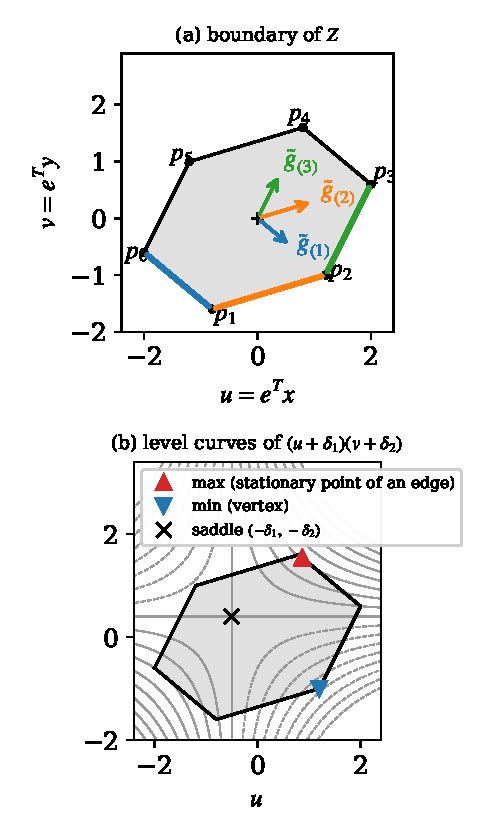
\includegraphics[height=0.6\textheight]{../fig/zonotope_kindle.pdf}
\caption{Lemma~\ref{lem:zonotope} and Algorithm~\ref{alg:exact} \DIFdelbeginFL \DIFdelFL{with three generators}\DIFdelendFL \DIFaddbeginFL \DIFaddFL{on Example~\ref{ex:alg}}\DIFaddendFL . (a) The generators \DIFaddbeginFL \DIFaddFL{$(2,-1)$, $(1,0)$, $(2,1)$}\DIFaddendFL , turned to the half-plane $u>0$ and sorted by angle; the boundary of $Z$ starts at \DIFdelbeginFL \DIFdelFL{$p_0=-\sum_k\tilde g_{(k)}$}\DIFdelendFL \DIFaddbeginFL \DIFaddFL{$p_0=-\sigma$}\DIFaddendFL , adds $2\tilde g_{(1)},2\tilde g_{(2)},2\tilde g_{(3)}$ (colored edges) and then subtracts them in the same order. (b) Level curves of $\varphi_\delta$ for \DIFdelbeginFL \DIFdelFL{$\delta=(0.5,-0.4)$ }\DIFdelendFL \DIFaddbeginFL \DIFaddFL{$\delta=(1,1)$, the vertex $(s,t)=(1,1)$ }\DIFaddendFL (dashed: negative values). Its only critical point is a saddle, so its extrema over $Z$ lie on the boundary\DIFdelbeginFL \DIFdelFL{: }\DIFdelendFL \DIFaddbeginFL \DIFaddFL{; }\DIFaddendFL here \DIFdelbeginFL \DIFdelFL{the minimum at a vertex and the maximum }\DIFdelendFL \DIFaddbeginFL \DIFaddFL{both are attained }\DIFaddendFL at \DIFdelbeginFL \DIFdelFL{the }\DIFdelendFL stationary \DIFdelbeginFL \DIFdelFL{point }\DIFdelendFL \DIFaddbeginFL \DIFaddFL{points }\DIFaddendFL of \DIFdelbeginFL \DIFdelFL{an edge}\DIFdelendFL \DIFaddbeginFL \DIFaddFL{edges}\DIFaddendFL . Algorithm~\ref{alg:exact} performs this walk for the four shifts $\delta=(x_rs,y_rt)$.}
\label{fig:zonotope}
\end{figure}

Let $[p,q]$ be an edge of the translated polygon $Z+\delta$, with direction $d=q-p$, parametrized as $p+\tau d$ with $\tau\in[0,1]$. Then
\[
\begin{gathered}\varphi_0(p+\tau d)=(p_u+\tau d_u)(p_v+\tau d_v)=P+B\tau+A\tau^2,\\ P=p_up_v,\quad B=p_ud_v+p_vd_u,\quad A=d_ud_v,\end{gathered}
\]
whose extrema over $[0,1]$ are attained at $\tau\in\{0,1\}$, with values $\varphi_0(p)$ and $\varphi_0(q)$, or, if $A\ne0$ and $\tau^*=-B/(2A)\in(0,1)$, at the stationary point, with value $P-B^2/(4A)$. This gives Algorithm~\ref{alg:exact}\DIFdelbegin \DIFdel{, where ``update $\ell,h$ with $w$'' stands for $\ell\gets\min(\ell,w)$, $h\gets\max(h,w)$}\DIFdelend .

\begin{algorithm}[H]
\caption{Exact multiplication of reduced affine forms}
\label{alg:exact}
\begin{algorithmic}[1]
\Require $\hat x = x_0+\sum_ix_i\eps_i+x_r\ex$, $\hat y = y_0+\sum_iy_i\eps_i+y_r\ey$
\Ensure $\hat z$ with $\hat x\hat y\in\hat z$ for all $e,\ex,\ey$, and $x_0y_0+c\pm z_r = x_0y_0+\rng N$
\State $\tilde g_{(1)},\dots,\tilde g_{(m)}\gets$ the nonzero $(x_i,y_i)$, turned to the half-plane $u>0$ and sorted by angle
\State $\sigma\gets\sum_{k=1}^m\tilde g_{(k)}$;\quad $\ell\gets+\infty$, $h\gets-\infty$
\For{$s\in\{-1,1\}$, $t\in\{-1,1\}$}
  \State $\delta\gets(x_rs,\,y_rt)$, $\kappa\gets x_0y_rt+y_0x_rs$
  \State $p\gets\delta-\sigma$ \Comment{vertex $p_0$ of~\eqref{eq:boundary}, translated by $\delta$}
  \State \DIFdelbegin \DIFdel{update $\ell,h$ with $\kappa+p_up_v$
  }\DIFdelend \DIFaddbegin \DIFadd{$\ell\gets\min(\ell,\,\kappa+p_up_v)$, $h\gets\max(h,\,\kappa+p_up_v)$
  }\DIFaddend \For{$j=1,\dots,2m$}
    \State $d\gets2\tilde g_{(j)}$ if $j\le m$, and $d\gets-2\tilde g_{(j-m)}$ otherwise
    \State $q\gets p+d$; \DIFdelbegin \DIFdel{update $\ell,h$ with $\kappa+q_uq_v$
    }\DIFdelend \DIFaddbegin \DIFadd{$\ell\gets\min(\ell,\,\kappa+q_uq_v)$, $h\gets\max(h,\,\kappa+q_uq_v)$
    }\DIFaddend \State $A\gets d_ud_v$, $B\gets p_ud_v+p_vd_u$
    \If{$A\ne0$ and $0<-B/(2A)<1$}
      \State \DIFdelbegin \DIFdel{update $\ell,h$ with $\kappa+p_up_v-B^2/(4A)$
    }\DIFdelend \DIFaddbegin \DIFadd{$w\gets\kappa+p_up_v-B^2/(4A)$; $\ell\gets\min(\ell,w)$, $h\gets\max(h,w)$
    }\DIFaddend \EndIf
    \State $p\gets q$
  \EndFor
\EndFor
\State $c\gets(\ell+h)/2$, $z_r\gets(h-\ell)/2$ (rounded outwards in a rigorous implementation)
\State \Return $\hat z = x_0y_0+c+e^T(y_0x+x_0y)+z_r\eps_z$
\end{algorithmic}
\end{algorithm}

Algorithm~\ref{alg:exact} works as follows (Figure~\ref{fig:zonotope}). Line~1 turns the generators to the half-plane $u>0$ and sorts them by angle, and line~2 computes their sum $\sigma$; both are done once, since the four polygons visited later are translates of the same polygon~\eqref{eq:boundary}. The outer loop visits the four vertices $(s,t)$ of $\U^2$, where the extrema of $N$ are attained (Lemma~\ref{lem:vertices}): with the error symbols fixed, $N(\cdot,s,t)$ is $\kappa$ plus $\varphi_0$ on the translate $Z+\delta$, by~\eqref{eq:Nst}. The walk starts at the vertex $p=\delta-\sigma$, which is $p_0$ translated by $\delta$, and the inner loop follows~\eqref{eq:boundary}: it adds the edge vectors $2\tilde g_{(1)},\dots,2\tilde g_{(m)}$ and then subtracts them in the same order, so that $p$ visits all the vertices of $Z+\delta$ and returns to the start. On each edge $[p,q]$, it evaluates $\varphi_0$ at the end $q$ (the start $p$ was evaluated in the previous step) and, if it lies inside the edge, at the stationary point. After the four walks, $\ell$ and $h$ are the endpoints of $\rng N$, and their midpoint and half-width give the new center shift $c$ and error term $z_r$.

\begin{theorem}
\label{thm:exact}
Algorithm~\ref{alg:exact} computes $\rng N$ exactly (in exact arithmetic) in $O(n\log n)$ time. Consequently, among all reduced affine forms with linear part $e^T(y_0x+x_0y)$ that enclose $\hat x\hat y$ over $\U^{n+2}$, the one returned by Algorithm~\ref{alg:exact} has the smallest error term $z_r$.
\end{theorem}
\begin{proof}
By Lemma~\ref{lem:vertices}, the endpoints of $\rng N$ are the extreme endpoints of the ranges of $N(\cdot,s,t)$, and by~\eqref{eq:Nst} and Lemma~\ref{lem:zonotope}, each of them is the range of $\kappa+\varphi_\delta$ over the boundary of $Z$, which the inner loop computes exactly. The generators are sorted once, in $O(n\log n)$ time, and each of the four walks along the $2m\le 2n$ edges takes $O(n)$ time. For the second statement, a reduced affine form with that linear part encloses $\hat x\hat y$ if and only if $[c-z_r,c+z_r]\supseteq\rng N$, by~\eqref{eq:product}; the narrowest such interval is $\rng N$.
\end{proof}

\begin{example}
\label{ex:alg}
Let \DIFdelbegin \DIFdel{$\hat x=1+\eps_1+\eps_2+\ex$ and $\hat y=2+\eps_1-\eps_2+\ey$}\DIFdelend \DIFaddbegin \DIFadd{$\hat x=1+\eps_1+2\eps_2+2\eps_3+\ex$ and $\hat y=1+\eps_2-\eps_3+\ey$}\DIFaddend , so that \DIFdelbegin \DIFdel{$n=2$ }\DIFdelend \DIFaddbegin \DIFadd{$n=3$ }\DIFaddend and $x_r=y_r=1$. The generators \DIFdelbegin \DIFdel{$(1,1)$ and $(1,-1)$ }\DIFdelend \DIFaddbegin \DIFadd{$(1,0)$, $(2,1)$ and $(2,-1)$ }\DIFaddend already lie in the half-plane $u>0$; sorted by angle, \DIFdelbegin \DIFdel{$\tilde g_{(1)}=(1,-1)$ and $\tilde g_{(2)}=(1,1)$, so $\sigma=(2,0)$ }\DIFdelend \DIFaddbegin \DIFadd{$\tilde g_{(1)}=(2,-1)$, $\tilde g_{(2)}=(1,0)$ and $\tilde g_{(3)}=(2,1)$, so $\sigma=(5,0)$ }\DIFaddend and $Z$ is the \DIFdelbegin \DIFdel{square with vertices $(-2,0)$, $(0,-2)$, $(2,0)$, $(0,2)$}\DIFdelend \DIFaddbegin \DIFadd{hexagon with vertices $(-5,0)$, $(-1,-2)$, $(1,-2)$, $(5,0)$, $(1,2)$, $(-1,2)$ (Figure~\ref{fig:zonotope}a)}\DIFaddend . For each vertex $(s,t)$ of $\U^2$, $\delta=(s,t)$ and \DIFdelbegin \DIFdel{$\kappa=t+2s$, and the walk along $Z+\delta$ gives the extrema of $uv$ below, where an asterisk marks a value attained at }\DIFdelend \DIFaddbegin \DIFadd{$\kappa=s+t$. For $(s,t)=(1,1)$, for instance, }\DIFaddend the \DIFdelbegin \DIFdel{stationary point of an edge(here, its midpoint) and the other values }\DIFdelend \DIFaddbegin \DIFadd{walk starts at $p=\delta-\sigma=(-4,1)$, and on the fourth edge, from $p=(6,1)$ to $q=(2,3)$ with $d=(-4,2)$, $\varphi_0(p+\tau d)=6+8\tau-8\tau^2$ reaches its maximum $8$ at $\tau^*=\tfrac12$, the point $(4,2)$, although it is $6$ at both ends of the edge. The four walks give the following extrema of $uv$; in this example all of them }\DIFaddend are attained at \DIFdelbegin \DIFdel{vertices}\DIFdelend \DIFaddbegin \DIFadd{stationary points of edges, at $\tau^*\in\{\tfrac14,\tfrac12,\tfrac34\}$}\DIFaddend :
\begin{center}
\small
\begin{adjustbox}{max width=\linewidth}\begin{tabular}{rrrrr}
\toprule
$(s,t)$ & $\kappa$ & $\min uv$ & $\max uv$ & $\kappa+[\min,\max]$ \\
\midrule
$(-1,-1)$ & \DIFdelbegin \DIFdel{$-3$ }\DIFdelend \DIFaddbegin \DIFadd{$-2$ }\DIFaddend & \DIFdelbegin \DIFdel{$-1$ }\DIFdelend \DIFaddbegin \DIFadd{$-\tfrac92$ }\DIFaddend & \DIFdelbegin \DIFdel{$4^*$ }\DIFdelend \DIFaddbegin \DIFadd{$8$ }\DIFaddend & \DIFdelbegin \DIFdel{$[-4,1]$ }\DIFdelend \DIFaddbegin \DIFadd{$[-\tfrac{13}2,6]$ }\DIFaddend \\
$(-1,1)$ & \DIFdelbegin \DIFdel{$-1$ }\DIFdelend \DIFaddbegin \DIFadd{$0$ }\DIFaddend & \DIFdelbegin \DIFdel{$-4^*$ }\DIFdelend \DIFaddbegin \DIFadd{$-8$ }\DIFaddend & \DIFdelbegin \DIFdel{$1$ }\DIFdelend \DIFaddbegin \DIFadd{$\tfrac92$ }\DIFaddend & \DIFdelbegin \DIFdel{$[-5,0]$ }\DIFdelend \DIFaddbegin \DIFadd{$[-8,\tfrac92]$ }\DIFaddend \\
$(1,-1)$ & \DIFdelbegin \DIFdel{$1$ }\DIFdelend \DIFaddbegin \DIFadd{$0$ }\DIFaddend & \DIFdelbegin \DIFdel{$-4^*$ }\DIFdelend \DIFaddbegin \DIFadd{$-8$ }\DIFaddend & \DIFdelbegin \DIFdel{$1$ }\DIFdelend \DIFaddbegin \DIFadd{$\tfrac92$ }\DIFaddend & \DIFdelbegin \DIFdel{$[-3,2]$ }\DIFdelend \DIFaddbegin \DIFadd{$[-8,\tfrac92]$ }\DIFaddend \\
$(1,1)$ & \DIFdelbegin \DIFdel{$3$ }\DIFdelend \DIFaddbegin \DIFadd{$2$ }\DIFaddend & \DIFdelbegin \DIFdel{$-1$ }\DIFdelend \DIFaddbegin \DIFadd{$-\tfrac92$ }\DIFaddend & \DIFdelbegin \DIFdel{$4^*$ }\DIFdelend \DIFaddbegin \DIFadd{$8$ }\DIFaddend & \DIFdelbegin \DIFdel{$[2,7]$ }\DIFdelend \DIFaddbegin \DIFadd{$[-\tfrac52,10]$ }\DIFaddend \\
\bottomrule
\end{tabular}\end{adjustbox}
\end{center}
Hence \DIFdelbegin \DIFdel{$\rng N=[-5,7]$}\DIFdelend \DIFaddbegin \DIFadd{$\rng N=[-8,10]$}\DIFaddend , $c=1$, \DIFdelbegin \DIFdel{$z_r=6$}\DIFdelend \DIFaddbegin \DIFadd{$z_r=9$}\DIFaddend , and, with the linear part \DIFdelbegin \DIFdel{$x_0y_0+e^T(y_0x+x_0y)=2+3\eps_1+\eps_2$}\DIFdelend \DIFaddbegin \DIFadd{$x_0y_0+e^T(y_0x+x_0y)=1+\eps_1+3\eps_2+\eps_3$}\DIFaddend , Algorithm~\ref{alg:exact} returns \DIFdelbegin \DIFdel{$\hat z=3+3\eps_1+\eps_2+6\eps_z$}\DIFdelend \DIFaddbegin \DIFadd{$\hat z=2+\eps_1+3\eps_2+\eps_3+9\eps_z$}\DIFaddend . The multiplication of Skalna and Hlad\'{\i}k encloses $R$ by its exact range \DIFdelbegin \DIFdel{$[-4,4]$ and adds $\pm(|y_0|x_r+|x_0|y_r)=\pm3$}\DIFdelend \DIFaddbegin \DIFadd{$[-8,8]$ and adds $\pm(|y_0|x_r+|x_0|y_r)=\pm2$}\DIFaddend , which gives \DIFdelbegin \DIFdel{$[-7,7]$ and $z_r=7$}\DIFdelend \DIFaddbegin \DIFadd{$[-10,10]$ and $z_r=10$}\DIFaddend . Here $2\min(|x_0|y_r,|y_0|x_r)=2$ is exactly the difference of widths, the largest one allowed by Corollary~\ref{cor:gain}.
\end{example}

\begin{remark}
Skalna and Hlad\'{\i}k reduce the computation of $R_{\max}$ to linear time by replacing the sorting with repeated median selection~\cite[Prop.~8]{skalna2017new}. Their argument uses the central symmetry of $Z$ and of $\varphi_0$, which locates the maximizer in the nonnegative quadrant. For the shifted products of~\eqref{eq:Nst} this symmetry is lost: the extrema can lie on any of the four monotone chains of the boundary, and these chains may cross the coordinate axes of the shifted product. A prune-and-search over each chain, in the spirit of~\cite[Prop.~8]{skalna2017new}, is a natural candidate, but it requires proving that $\varphi_\delta$ is unimodal along each chain, including the parts where its factors have opposite signs, and we leave a linear-time version of Algorithm~\ref{alg:exact} open. In practice, the $O(n\log n)$ version is the one recommended in~\cite{skalna2017new} for moderate $n$, and in our implementation the sorting is shared by the four vertices.
\end{remark}

\begin{remark}
When $x_r=y_r=0$, $N=Q$ and E gives the exact range of $\hat x\hat y - x_0y_0 - e^T(y_0x+x_0y)$; over a box, this is the narrowest residual of a linear relaxation of the product of two affine functions with the given slopes. All the multiplication formulae above keep the linear part~\eqref{eq:product}; choosing another linear part, as in the min-range approximations of~\cite{stolfi1997self,skalna2013minrange}, is a different problem that we do not consider.
\end{remark}

\section{A hierarchy of multiplication formulae}
\label{sec:hierarchy}

Denote by $[\hat z]_F$ the interval $[c-z_r,c+z_r]$ of formula $F$.

\begin{propo}
\label{prop:chain}
For all operands, $[\hat z]_E \subseteq [\hat z]_{SH}\subseteq[\hat z]_S\subseteq[\hat z]_T$.
\end{propo}
\begin{proof}
$[\hat z]_E=\rng N$ is contained in every valid enclosure. The inclusions $[\hat z]_{SH}\subseteq[\hat z]_S\subseteq[\hat z]_T$ follow from~\cite[Prop.~3]{skalna2017new}. The first one holds because the part of $[\hat z]_S$ that does not come from $|y_0|x_r+|x_0|y_r$ is a valid enclosure of $R$, which SH replaces by its exact range, and the second because the radius of S is that of T minus $\tfrac12|x|^T|y|$ and its center moves by $\tfrac12x^Ty$, with $|\tfrac12x^Ty|\le\tfrac12|x|^T|y|$. We will also use the identity
\[
\begin{aligned}&(\|x\|_1+x_r)(\|y\|_1+y_r) - \tfrac12|x|^T|y|\\ &\quad= \tfrac12|x|^T|y|+\sum_{i\ne j}|x_iy_j| + x_r\|y\|_1+y_r\|x\|_1+x_ry_r .\end{aligned}
\]
\end{proof}

The difference between E and SH comes from the terms $x_0y_r\ey$ and $y_0x_r\ex$, which SH bounds separately. When one of the operands has no error, this separation costs nothing.

\begin{propo}
\label{prop:oneerror}
If $x_r=0$ or $y_r=0$, then $[\hat z]_E=[\hat z]_{SH}$.
\end{propo}
\begin{proof}
Let $y_r=0$, so that $N = y_0x_r\ex + R$ with $R(e,\ex)=(e^Tx+x_r\ex)\,e^Ty$. Since $R$ is affine in $\ex$ for fixed $e$, its maximum over $\U^{n+1}$ is attained at some $(e^*,\ex^*)$ with $\ex^*\in\{-1,1\}$, and since $R(-e,-\ex)=R(e,\ex)$, also at $(-e^*,-\ex^*)$. Choosing the one with $\ex^*=\operatorname{sign}(y_0)$ (either, if $y_0=0$) gives $N = |y_0|x_r + R_{\max}$, which is the upper bound of $[\hat z]_{SH}$. The same argument applies to the lower bound, and to $x_r=0$.
\end{proof}

When both operands carry errors, E can be narrower than SH, but by a bounded factor. Denote $A=|y_0|x_r+|x_0|y_r$ and, for the two pairs of opposite vertices of $\U^2$, $\Lambda_\alpha=|x_0y_r+y_0x_r|$, the value of $|x_0y_r\ey+y_0x_r\ex|$ at $(\ex,\ey)=\pm(1,1)$, and $\Lambda_\beta=|x_0y_r-y_0x_r|$, its value at $\pm(1,-1)$, so that $\max(\Lambda_\alpha,\Lambda_\beta)=A$.

\begin{lemma}
\label{lem:classes}
The maximum of $R$ over $\U^{n+2}$ is attained at a point with $(\ex,\ey)=(1,1)$, and its minimum at a point with $(\ex,\ey)=(1,-1)$.
\end{lemma}
\begin{proof}
Write $R=(u+x_r\ex)(v+y_r\ey)$ with $(u,v)=(e^Tx,e^Ty)$. Since $R(0,0,0)=0$, $\max R\ge0$. If $\max R=0$, it is attained at $(e,\ex,\ey)=(0,1,1)$, where $R=x_ry_r\ge0$. Otherwise, at a maximizer both factors have the same sign, and since $R(-e,-\ex,-\ey)=R(e,\ex,\ey)$, we may assume that both are positive. Increasing $\ex$ and $\ey$ to $1$ does not decrease them, because $x_r,y_r\ge0$, so $R$ does not decrease and the maximum is also attained with $(\ex,\ey)=(1,1)$. The argument for the minimum is the same: if $\min R=0$, it is attained at $(0,1,-1)$, where $R=-x_ry_r\le0$; otherwise, at a minimizer the factors have opposite signs, we may assume that the first one is positive, and moving $(\ex,\ey)$ to $(1,-1)$ increases the first factor and decreases the second, so that $R$ does not increase.
\end{proof}

\begin{propo}
\label{prop:32}
For all operands, $\wid[\hat z]_E\ \ge\ \wid\rng R+\Lambda_\alpha+\Lambda_\beta$ and
\[
\wid[\hat z]_E\ \le\ \wid[\hat z]_{SH}\ \le\ \tfrac32\,\wid[\hat z]_E .
\]
The constant $3/2$ cannot be improved.
\end{propo}
\begin{proof}
Write $N=L+R$ with $L=x_0y_r\ey+y_0x_r\ex$, and let $p=(e,\ex,\ey)$. Since $R(-p)=R(p)$ and $L(-p)=-L(p)$, one of $N(p)$, $N(-p)$ is at least $R(p)+|L(p)|$ and the other is at most $R(p)-|L(p)|$; hence
\begin{equation}
\label{eq:pm}
\begin{gathered}\max N\ \ge\ R(p)+|L(p)|,\qquad \min N\ \le\ R(p)-|L(p)|\\ \text{for every } p\in\U^{n+2}.\end{gathered}
\end{equation}
Taking $p$ as the maximizer of $R$ given by Lemma~\ref{lem:classes}, where $|L(p)|=\Lambda_\alpha$, and then as its minimizer, where $|L(p)|=\Lambda_\beta$, gives $\wid[\hat z]_E=\max N-\min N\ge\wid\rng R+\Lambda_\alpha+\Lambda_\beta\ge\wid\rng R+A$. Taking in~\eqref{eq:pm} the same point $p=(0,\ex,\ey)$ for both bounds, with the vertex $(\ex,\ey)$ where $|L|=A$, gives $\wid[\hat z]_E\ge 2A$. Since $\wid[\hat z]_{SH}=\wid\rng R+2A$,
\[
\wid[\hat z]_{SH}\ \le\ \tfrac32\max\big(\wid\rng R+A,\ 2A\big)\ \le\ \tfrac32\,\wid[\hat z]_E ,
\]
where the first inequality is checked separately for $\wid\rng R\ge A$ and $\wid\rng R\le A$. The lower bound $\wid[\hat z]_E\le\wid[\hat z]_{SH}$ is Proposition~\ref{prop:chain}, and Example~\ref{ex:32} attains the ratio $3/2$.
\end{proof}

\begin{example}
\label{ex:32}
Let $n=0$, $\hat x = -1+\ex$ and $\hat y = 1+\ey$, i.e., $x\in[-2,0]$ and $y\in[0,2]$. Then $N = -\ey+\ex+\ex\ey$, whose values at the four vertices are $1,1,1,-3$, so $[\hat z]_E=[-3,1]$ and $\hat x\hat y\in -1+[-3,1]=[-4,0]$, the exact range of $xy$. SH gives $\rng R=[-1,1]$ and $|y_0|x_r+|x_0|y_r = 2$, so $[\hat z]_{SH}=[-3,3]$ and $\hat x\hat y\in[-4,2]$: the width ratio is $3/2$.
\end{example}

The lower bound of Proposition~\ref{prop:32} also tells when E can improve on SH, and by how much.

\begin{corollary}
\label{cor:gain}
For all operands,
\[
0\ \le\ \wid[\hat z]_{SH}-\wid[\hat z]_E\ \le\ 2\min\big(|x_0|\,y_r,\ |y_0|\,x_r\big).
\]
In particular, $[\hat z]_E=[\hat z]_{SH}$ whenever one of the operands has no error ($x_r=0$ or $y_r=0$) or a zero center ($x_0=0$ or $y_0=0$).
\end{corollary}
\begin{proof}
$\wid[\hat z]_{SH}=\wid\rng R+2A$ and, by Proposition~\ref{prop:32}, $\wid[\hat z]_E\ge\wid\rng R+\Lambda_\alpha+\Lambda_\beta$. Since $\Lambda_\alpha+\Lambda_\beta = |a+b|+|a-b| = 2\max(|a|,|b|)$ and $A=|a|+|b|$, with $a=x_0y_r$ and $b=y_0x_r$, the difference is at most $2A-2\max(|a|,|b|)=2\min(|a|,|b|)$.
\end{proof}

The bound is attained in most cases: in 100\,000 random products with $n\le6$ and nonzero bound, the difference was equal to $2\min(|x_0|y_r,|y_0|x_r)$ in 68\% of them, and its median ratio to the bound was 1. E is therefore useful when \emph{both} operands carry errors and are \emph{both} away from zero, and its relative gain, at most $1/3$ of $\wid[\hat z]_{SH}$ by Proposition~\ref{prop:32}, is largest when $|x_0|y_r$ and $|y_0|x_r$ are comparable and large with respect to the width of $\rng R$, i.e., when the errors and the centers of the operands dominate their noise coefficients. This is the typical situation of products of subexpressions that have accumulated errors in previous nonlinear operations, such as a square $\hat v\cdot\hat v$ of a nonlinear form, for which $|x_0|y_r=|y_0|x_r$.

\begin{propo}
\label{prop:square}
For the square of a form, $\rng N_2 = [-2|x_0|x_r,\ 2|x_0|x_r+(\|x\|_1+x_r)^2]$ whenever $x_r\le\|x\|_1$; that is, SH applied to $\hat x\hat x$ with the shared error symbol is exact. When $x_r=0$, both SH and E give $[0,\|x\|_1^2]$.
\end{propo}
\begin{proof}
Write $u=e^Tx$, which ranges over $[-\|x\|_1,\|x\|_1]$. The interval is an enclosure of $\rng N_2$, since $(u+x_r\ex)^2\in[0,(\|x\|_1+x_r)^2]$ and $|2x_0x_r\ex|\le2|x_0|x_r$. Its upper end is attained with $\ex=\sigma$ and $u=\sigma\|x\|_1$, where $\sigma=\operatorname{sign}(x_0)$ ($\sigma=1$ if $x_0=0$). Its lower end is attained with $\ex=-\sigma$ and $u=\sigma x_r$, which is a value of $u$ because $x_r\le\|x\|_1$, so that $u+x_r\ex=0$ and $N_2=-2|x_0|x_r$.
\end{proof}
The SH enclosure of a square is not new: with $r=\|x\|_1+x_r$, it is the Chebyshev linearization of $t\mapsto t^2$ over the range $[x_0-r,x_0+r]$ of $\hat x$, $t^2\in 2x_0t-x_0^2+[0,r^2]$, which is the usual way of enclosing univariate functions in AA~\cite{stolfi1997self}. The radius of S for a square exceeds that of SH by $\tfrac12(\|x\|_1+x_r)^2-\tfrac12x^Tx$, which approaches $\tfrac12(\|x\|_1+x_r)^2$, half the width of the exact range of the quadratic part, when the noise coefficients are spread over many symbols. Products and squares are thus two separate places where S loses with respect to the exact ranges, and in a solver both matter (Section~\ref{sec:solver}).

\paragraph{The standard multiplication is AF2 with re-centering.} The next result relates formula S to AF2.

\begin{propo}
\label{prop:af2}
Let $\hat x$, $\hat y$ be AF2 forms without one-sided terms, i.e., reduced affine forms with $\eps_\pm$ as error symbol. The AF2 product~\cite{messine2002extentions}
\[
\begin{gathered}x_0y_0 + e^T(y_0x+x_0y) + k_1\eps_\pm + k_2\eps_+ + k_3\eps_-,\\ k_2=\sum_{x_iy_i>0}x_iy_i,\quad k_3=\sum_{x_iy_i<0}|x_iy_i|,\end{gathered}
\]
\[
k_1 = |x_0|y_r+|y_0|x_r+\sum_{i\ne j}|x_iy_j| + x_r\|y\|_1+y_r\|x\|_1+x_ry_r,
\]
becomes the product given by formula S when $k_2\eps_+$ and $k_3\eps_-$ are replaced by their centers and radii, $k_2\eps_+\in \tfrac{k_2}{2}+\tfrac{k_2}{2}[-1,1]$ and $k_3\eps_-\in-\tfrac{k_3}{2}+\tfrac{k_3}{2}[-1,1]$.
\end{propo}
\begin{proof}
The re-centered form has center shift $\tfrac12(k_2-k_3)=\tfrac12x^Ty$ and error radius $k_1+\tfrac12(k_2+k_3) = k_1+\tfrac12|x|^T|y|$, which equals $z_r$ of formula S by the identity in the proof of Proposition~\ref{prop:chain}.
\end{proof}

Thus S and AF2 have the same width after one product, and they differ only in the next operations, where AF2 carries the offsets of $\eps_+$ and $\eps_-$. Among residual intervals of a given radius, a zero-centered one minimizes the width propagated through a product with another interval: if $\mathbf r=[r_c-\rho,r_c+\rho]$ and $\mathbf y$ is an interval with $Y=\max_{y\in\mathbf y}|y|$, then $\wid(\mathbf r\mathbf y)\ge 2\rho Y$, with equality for $r_c=0$. This explains why S is tighter than AF2 in compositions of products (Section~\ref{sec:experiments}).

\begin{remark}
S can be much wider than SH even without errors: for $\hat x=\eps_1+\eps_2$ and $\hat y=\eps_1-\eps_2$, S (and AF2) give an enclosure of width $6$, while SH and E give $2$, the width of the exact range $[-1,1]$ of $\eps_1^2-\eps_2^2$.
\end{remark}

\section{Rigorous floating-point implementation}
\label{sec:rigor}

A floating-point implementation of Algorithm~\ref{alg:exact} must return an interval that contains $\rng N$. Two points need care.
\begin{itemize}
\item \emph{Angular order.} An incorrect order between two almost parallel generators would produce a path that cuts through the interior of $Z$ and could underestimate the range. The order is decided by the sign of $u_1v_2-v_1u_2$, evaluated in double precision with a forward error filter~\cite{shewchuk1997adaptive}: if $|\mathrm{fl}(u_1v_2)-\mathrm{fl}(v_1u_2)|$ exceeds $4\cdot2^{-52}(|\mathrm{fl}(u_1v_2)|+|\mathrm{fl}(v_1u_2)|)$ and neither product underflows, its sign is the exact one; otherwise the expression is evaluated in quadruple precision, where the two products are exact and the subtraction preserves the sign. Flipping a generator to the half-plane $u>0$ is exact.
\item \emph{Boundary walk.} The vertices and the values on the edges are computed in double precision, and the resulting interval is widened by an a priori bound of the rounding errors. Let $m$ be the number of generators (including $(x_r,0)$ and $(0,y_r)$ for SH), $U=|\delta_1|+3\sum_k|u_k|$ and $V=|\delta_2|+3\sum_k|v_k|$ (with $\delta=0$ for SH), which bound $|u|$ and $|v|$ at every computed or exact vertex, partial sum and edge point. Each vertex is obtained with at most $3m+2$ additions, so its error is at most $(3m+2)\,\eps_m U$ in $u$ and $(3m+2)\,\eps_m V$ in $v$, with $\eps_m=2^{-52}$, which bounds the error of one operation in any rounding mode~\cite{higham2002accuracy}. On an edge $[p,p+d]$ with $d=\pm2\tilde g_{(j)}$ (exact), the value at the stationary point is $P-B^2/(4A)$, with the notation above; since the stationary point is in $(0,1)$, $|B|<2|A|$, and $|P|,|A|\le UV$, $|B|\le2UV$, so each evaluated value has a rounding error of $O(\eps_m UV)$, and a wrong decision on whether the stationary point lies in $(0,1)$ changes the value by $O(\eps_m UV)$ as well. Adding the constant $\kappa$ and the term $|y_0|x_r+|x_0|y_r$ of SH, we widen the interval by $(8m+64)\,\eps_m\,(UV+|x_0|y_r+|y_0|x_r)$ and round its endpoints outwards. This widening is of the order of $10^{-13}$ times the width of the enclosure.
\end{itemize}
Our implementation sorts the generators once per product, walks the four shifted polygons of E in a single pass, and allocates no memory per product. For E, when $\min(|x_0|y_r,|y_0|x_r)=0$, it runs the single walk of SH, which gives the same interval by Corollary~\ref{cor:gain}.

For squares, both SH and E use the SH bound, that is, the Chebyshev linearization of $t^2$, which is exact when $x_r\le\|x\|_1$ (Proposition~\ref{prop:square}). The center and the radius of the enclosure are then added to the reduced affine form with the usual outward rounding of the linear part.

\section{Experiments}
\label{sec:experiments}

\subsection{Range enclosures}

The formulae S, SH and E and AF2 were first implemented in Python, in double precision without outward rounding, on the representation in the variable space described in the introduction (a linear function of the variables plus a residual interval), in which a product has the linear part of~\eqref{eq:product} for all the formulae. Univariate functions are enclosed by the same Chebyshev linearization in all methods, so that the differences come only from the products. Every enclosure was checked by sampling, and the inclusions of Proposition~\ref{prop:chain} were verified on 2000 random products. Exact ranges were computed with IbexOpt~\cite{chabert2009}. The code, the data and the scripts that produce the tables are available at \url{https://github.com/rilianx/raa-affine-arithmetic}.

\paragraph{Random products.} Table~\ref{tab:random} reports single products of random forms over $[-1,1]^n$ (so that the variables are the noise symbols), with standard normal coefficients, centers of standard deviation 2, and error radii $|\mathcal N(0,1)|\rho$. Without errors ($\rho=0$), SH and E coincide, as they compute the exact range of $Q$. With errors, E is strictly narrower than SH in every product, and SH is up to 1.37 times wider than E for $n=2$; the mean advantage decreases with $n$, since the gain is bounded by $2\min(|x_0|y_r,|y_0|x_r)$ (Corollary~\ref{cor:gain}), while the width of the quadratic part, which both compute exactly, grows with $n$. S is 1.4--2.0 times wider than E.

\begin{table}[H]
\centering
\caption{Single products of random forms with $n$ variables: mean width of the enclosures of rules S and SH relative to E, and maximum of SH/E. $\rho$ scales the error radii of the operands; 500 products per row.}
\label{tab:random}
\small
\begin{adjustbox}{max width=\linewidth}\begin{tabular}{rrrrr}
\toprule
 & & \multicolumn{2}{c}{Mean width / E} & \\
\cmidrule(lr){3-4}
$n$ & $\rho$ & S & SH & max SH/E \\
\midrule
2 & 0.0 & 1.656 & 1.000 & 1.000 \\
 & 0.1 & 1.504 & 1.019 & 1.138 \\
 & 1.0 & 1.366 & 1.070 & 1.370 \\
\midrule
5 & 0.0 & 1.901 & 1.000 & 1.000 \\
 & 0.1 & 1.847 & 1.007 & 1.048 \\
 & 1.0 & 1.630 & 1.036 & 1.261 \\
\midrule
10 & 0.0 & 1.961 & 1.000 & 1.000 \\
 & 0.1 & 1.919 & 1.002 & 1.013 \\
 & 1.0 & 1.781 & 1.012 & 1.119 \\
\midrule
20 & 0.0 & 1.975 & 1.000 & 1.000 \\
 & 0.1 & 1.964 & 1.000 & 1.004 \\
 & 1.0 & 1.902 & 1.004 & 1.025 \\
\bottomrule
\end{tabular}\end{adjustbox}
\end{table}

\paragraph{Test functions of Skalna and Hlad\'{\i}k.} Table~\ref{tab:sh} repeats the range-bounding experiment of~\cite[Table~3]{skalna2017new}: the nine test functions are evaluated over the same boxes, with integer powers computed as repeated products with the corresponding formula, and the overestimation $1-\wid(f^H)/\wid(\hat f)$ of the exact range $f^H$, computed with IbexOpt, is reported. For $f_1$--$f_5$, our values of S and SH agree with those of~\cite{skalna2017new} up to rounding, which validates our implementation of their formulae. For Matyas, the widths of the enclosures agree with theirs (the ratio between the widths of formulae T and S is $0.74$ in both cases), but the overestimations reported in~\cite{skalna2017new} (96--97\%) correspond to a reference range of width about 6, whereas the range of $f_7$ over $[-10,10]^2$ is $[0,100]$. For Leon, the 9\% reported for SH is below what E attains with any of the evaluation orders of the powers that we tried, so the expressions must have been evaluated in another form; the remaining differences, for $f_6$, $f_8$ and $f_9$, are presumably of the same origin.

\begin{table}[H]
\centering
\caption{Overestimation (\%) of the exact range of the test functions of~\cite{skalna2017new}, with integer powers computed as repeated products.}
\label{tab:sh}
\small
\begin{adjustbox}{max width=\linewidth}\begin{tabular}{llrrr}
\toprule
Function & Box & S & SH & E \\
\midrule
$f_1$ Beale & $[-5,5]^2$ & 49.9 & 49.1 & 48.8 \\
$f_2$ Booth & $[-10,10]^2$ & 35.8 & 19.9 & 19.9 \\
$f_3$ Colville & $[-10,10]^4$ & 36.6 & 33.2 & 13.6 \\
$f_4$ Dixon ($n=5$) & $[-5,5]^5$ & 36.6 & 33.1 & 13.6 \\
$f_5$ Goldstein--Price & $[-2,2]^2$ & 99.1 & 98.6 & 98.1 \\
$f_6$ Leon & $[-1.2,1.2]^2$ & 39.1 & 28.4 & 24.4 \\
$f_7$ Matyas & $[-10,10]^2$ & 32.4 & 32.4 & 32.4 \\
$f_8$ Rosenbrock ($n=4$) & $[-5,10]^4$ & 47.5 & 36.0 & 32.3 \\
$f_9$ Six-hump camel & $[-5,5]^2$ & 57.4 & 39.9 & 39.9 \\
\bottomrule
\end{tabular}\end{adjustbox}
\end{table}

E is much tighter than SH for Colville and Dixon (13.6\% instead of 33\%), and also for Leon and Rosenbrock. These functions contain squares $(x_i^2-x_j)^2$ computed as products $\hat v\cdot\hat v$ of a form that carries the error of the product $x_i\cdot x_i$ and whose center is far from zero, which is the most favorable case of Corollary~\ref{cor:gain}; in Booth and Matyas, every product has an operand without error, and E and SH coincide.

\paragraph{Controlled products and benchmark constraints.} Finally, we consider expressions in three variables evaluated over random boxes inside $[-10,10]^3$ of three sizes, with widths in $[0.01,0.1]$, $[0.1,1]$ and $[1,10]$: four controlled products, Case~1 $(x_1+2x_2+3x_3)(4x_1+5x_2+6x_3)$, Case~2 $(x_1+2x_2^2+3x_3)(4x_1+5x_2+6x_3^2)$, Case~3 $(x_1+2x_2x_3)(3x_2+4x_1x_3)$ and Case~4 $(x_1+2x_2)(3x_2+4x_3)(5x_3+6x_1)$, the same expressions with some coefficients negated (Cases 1m--4m), and four constraints with products of nonlinear factors taken from a benchmark of nonlinear systems~\cite{coprin} (Trigexp1, two constraints of Trigexp2, and Pramanik). The quality of a method is measured by its gap $100\,(W-W^*)/W^*$, where $W$ is the width of its residual and $W^*$ the exact width of the range of $f(x)-L(x)$ over the box, $L$ being the linear part of the products, computed with IbexOpt. Table~\ref{tab:expressions} shows Cases~1--4, Case~1m and the four constraints; Cases~2m--4m behave as Cases~2--4 (all the results are in the repository).

\begin{table}[H]
\centering
\caption{Controlled products and constraints from a benchmark of nonlinear systems: mean gap (\%) of each method with respect to the optimal residual width for its own linear part, over all boxes (100 per size for the controlled cases and Trigexp1, 50 for the other constraints), number of boxes where E is strictly narrower than SH, and largest width reduction of E with respect to SH.}
\label{tab:expressions}
\small
\setlength{\tabcolsep}{4pt}
\begin{adjustbox}{max width=\linewidth}\begin{tabular}{lrrrrrr}
\toprule
 & \multicolumn{4}{c}{Mean gap (\%)} & \multicolumn{2}{c}{E vs SH} \\
\cmidrule(lr){2-5}\cmidrule(lr){6-7}
Expression & AF2 & S & SH & E & E $<$ SH & max red. \\
\midrule
Case 1 & 57.3 & 57.3 & 0.0 & 0.0 & 0/300 & 0.0\% \\
Case 1m & 121.8 & 121.8 & 0.0 & 0.0 & 0/300 & 0.0\% \\
Case 2 & 49.1 & 49.1 & 23.2 & 21.1 & 300/300 & 15.1\% \\
Case 3 & 42.5 & 42.5 & 9.5 & 7.4 & 300/300 & 11.0\% \\
Case 4 & 92.4 & 88.5 & 34.2 & 34.2 & 0/300 & 0.0\% \\
\midrule
Trigexp1 & 41.7 & 41.7 & 30.6 & 30.4 & 285/300 & 4.1\% \\
Trigexp2 (1) & 10.1 & 10.1 & 6.0 & 5.8 & 150/150 & 2.2\% \\
Trigexp2 (2) & 110.9 & 110.9 & 76.3 & 76.3 & 0/150 & 0.0\% \\
Pramanik & 531.7 & 531.7 & 487.3 & 487.3 & 0/100 & 0.0\% \\
\bottomrule
\end{tabular}\end{adjustbox}
\end{table}

For affine operands (Cases~1 and 1m), SH and E are exact, while AF2 and S lose 57\%, and 122\% when the bilinear terms cancel (Case~1m). When the operands carry errors, E is strictly narrower than SH in all the boxes of Cases~2 and~3 (and of 2m and 3m), by 1.8\% on average and by up to 15.1\% (20.5\% in Case~2m; one-sided Wilcoxon signed-rank test over the 2400 controlled boxes, $p=4\times10^{-198}$). The advantage grows with the size of the box: in the largest boxes, the mean gap of Case~3 drops from 7.6\% with SH to 2.8\% with E. In Case~4, each product has an operand without error, and E and SH coincide, as stated by Proposition~\ref{prop:oneerror}; S is tighter than AF2 in this chained product, as expected from Proposition~\ref{prop:af2}. On the benchmark constraints, E is narrower than SH in 435 of the 700 boxes and never wider, but only by 0.1\% on average and by at most 4.1\%: the residuals of these constraints are dominated by the linearization of the univariate functions, and the factors of their products are sines, whose centers are close to zero when they are linearized over wide intervals, and exponentials or affine expressions without error.

\subsection{Implementation in Ibex}
\label{sec:ibex}

We implemented SH and E in the affine arithmetic of the Ibex library~\cite{chabert2009,ibexaffine} (model fAF2 of its affine plugin), whose multiplication and square are those of formula S, with the rounding errors of each operation accumulated in the error term. Only the enclosure $[c-z_r,c+z_r]$ of $N$ (or $N_2$) changes: the linear part, its rounding errors and the way they are added to the error term are those of fAF2. Note that S is exact for the products and squares of the variables themselves, whose forms have a single noise symbol and no error, so that the formulae differ only for compound factors.

\paragraph{Validation.} The implementation was checked against the exact range of $N$ computed with rational arithmetic on 86\,000 random products, including almost parallel generators and coefficients from $10^{-6}$ to $10^6$, without any violation, and with the containment test of the RAA-K experiments of the Ibex affine plugin~\cite{ibexaffine}, which evaluates 180\,000 random functions of nine families at sampled points with interval arithmetic: no enclosure was violated, while the test detects violations when the error term is artificially reduced by 10\%.

\paragraph{Cost.} Table~\ref{tab:cost} gives the time per product of the multiplication of fAF2 (S) and of SH and E. The exact-range multiplications cost 2.3--5.4 times as much as S; E costs about 10\% more than SH when the operands carry errors, and the same otherwise. In the solver experiments below, this overhead is a small fraction of the time per node.

\begin{table}[H]
\centering
\caption{Time per product ($\mu$s) in the affine arithmetic of Ibex, for random forms with $n$ noise symbols, with and without error terms in the operands (C++, \texttt{-O2}, one core).}
\label{tab:cost}
\small
\begin{adjustbox}{max width=\linewidth}\begin{tabular}{rrrrrrr}
\toprule
 & \multicolumn{3}{c}{Without errors} & \multicolumn{3}{c}{With errors} \\
\cmidrule(lr){2-4}\cmidrule(lr){5-7}
$n$ & S & SH & E & S & SH & E \\
\midrule
2 & 0.09 & 0.31 & 0.30 & 0.09 & 0.34 & 0.30 \\
5 & 0.15 & 0.41 & 0.42 & 0.16 & 0.48 & 0.42 \\
10 & 0.25 & 0.66 & 0.67 & 0.25 & 0.76 & 0.71 \\
20 & 0.47 & 1.47 & 1.61 & 0.45 & 1.59 & 1.54 \\
50 & 1.07 & 4.65 & 4.60 & 1.16 & 4.79 & 4.65 \\
100 & 2.15 & 10.56 & 10.35 & 2.13 & 10.70 & 10.61 \\
\bottomrule
\end{tabular}\end{adjustbox}

\end{table}

\subsection{Global optimization with IbexOpt}
\label{sec:solver}

We replaced the multiplication and the square of fAF2 by those of SH and E in IbexOpt~\cite{chabert2009}, configured with the affine linear relaxation of~\cite{ninin2015reliable}, in which every constraint and the objective are linearized over each box by evaluating them with reduced affine forms, the lsmear bisection heuristic~\cite{araya2017}, precision $10^{-7}$ on the variables and relative precision $10^{-6}$ on the objective. All the other components of the solver are unchanged, so that S, SH and E differ only in the enclosures of products and squares. We used four sets of instances:
\begin{itemize}
\item \emph{synq}: 78 synthetic problems with 3 to 10 variables, whose objective is a sum of products of random linear forms plus a linear term, under random linear constraints; every product has compound factors without errors, the case where SH and E are exact and S is not.
\item \emph{synt}: 24 synthetic problems whose objective contains products of linear forms with univariate functions ($\sin$, $\cos$, $\exp$, $\ln$) and products of two univariate functions, such as $\cos(\cdot)\exp(\cdot)$, whose factors both carry linearization errors.
\item \emph{synp}: 18 synthetic problems whose objective is a sum of products of two quadratic functions with nonzero constant terms, so that both factors carry errors and have nonzero centers, the favorable case of Corollary~\ref{cor:gain}.
\item \emph{medium+hard}: the 38 instances of the medium and hard sets of the optimization benchmark distributed with Ibex, taken from the COCONUT library~\cite{coconut}.
\end{itemize}
Each run used one core, with four simultaneous runs on the same machine, and the time limits of Table~\ref{tab:solver}. Table~\ref{tab:solver} reports the number of instances solved within the limit and, over the instances solved by the three multiplications, the geometric means of the numbers of nodes and of the CPU times relative to S, and the comparison of E with SH. The three multiplications found the same optimum, within the precision, on every instance solved by all of them.

\begin{table}[H]
\centering
\caption{IbexOpt with the multiplications S (standard, the one of fAF2), SH and E: instances solved within the time limit $t_{\max}$ (s), geometric means of nodes and CPU time relative to S over the instances solved by all three, geometric mean of the nodes of E relative to SH, and numbers of instances where E needs at least 1\% fewer / more nodes than SH. SH$^\dagger$: SH for products, with the square of S (ablation; synq has no squares).}
\label{tab:solver}
\small
\setlength{\tabcolsep}{3.5pt}
\begin{adjustbox}{max width=\linewidth}\begin{tabular}{lrrrrrr}
\toprule
 & & & \multicolumn{4}{c}{Solved} \\
\cmidrule(lr){4-7}
Set & Inst. & $t_{\max}$ & S & S$^+$ & SH & E \\
\midrule
synq & 78 & 300 & 45 & 45 & 61 & 60 \\
synt & 24 & 60 & 19 & 19 & 20 & 20 \\
synp & 18 & 60 & 18 & 18 & 18 & 18 \\
Ibex medium+hard & 38 & 200 & 33 & 33 & 35 & 34 \\
\bottomrule
\end{tabular}\end{adjustbox}

\medskip
\begin{adjustbox}{max width=\linewidth}\begin{tabular}{lrrrrrrr}
\toprule
 & \multicolumn{3}{c}{Nodes / S$^+$} & \multicolumn{2}{c}{CPU / S$^+$} & \multicolumn{2}{c}{E vs SH} \\
\cmidrule(lr){2-4}\cmidrule(lr){5-6}\cmidrule(lr){7-8}
Set & S & SH & E & SH & E & nodes & $<$/$>$ \\
\midrule
synq & 1.00 & 0.26 & 0.26 & 0.29 & 0.31 & 0.998 & 4/9 \\
synt & 1.00 & 0.67 & 0.62 & 0.69 & 0.70 & 0.926 & 11/1 \\
synp & 1.00 & 0.83 & 0.79 & 0.91 & 0.88 & 0.961 & 8/2 \\
Ibex medium+hard & 1.07 & 0.98 & 0.92 & 0.87 & 0.91 & 0.942 & 10/1 \\
\bottomrule
\end{tabular}\end{adjustbox}

\end{table}

\paragraph{Exact-range multiplications versus S.} On synq, SH and E solve 61 instances instead of 45 and need about four times fewer nodes (0.26) and 3.4 times less time on the instances solved by S; on the 17 instances that none of them solves, the final gap between the bounds of the objective is reduced to 37\% of that of S. This is the effect of computing the quadratic part of the products exactly: the factors are linear forms of many variables, for which S overestimates the range of the product up to a factor 2 (Table~\ref{tab:random}). On synt and synp, the reduction is 33\% and 17\% of the nodes, and on the classical benchmark it is 8--11\%, with two more instances solved (chem and chem-1, which S does not solve within 200 s). The last column of SH$^\dagger$ explains the difference: with the square of S, SH does not reduce the nodes at all on medium+hard (1.00), so that the whole improvement on these instances comes from the squares of compound expressions, such as $(x_i-x_j)^2$, for which S is almost twice as wide as the Chebyshev square (Proposition~\ref{prop:square}). Most products and squares in these instances involve single variables, for which S is already exact. In synt and synp, on the contrary, the squares are squares of variables, and the ablation changes nothing.

\paragraph{E versus SH.} E coincides with SH on synq, where the factors carry only rounding errors (geometric mean 1.000, with differences of more than 1\% in 7 of 45 instances, in both directions), and improves on SH exactly where Corollary~\ref{cor:gain} predicts: on synt and synp, where both factors carry errors and have nonzero centers, E needs 7\% and 4\% fewer nodes than SH, it needs fewer nodes in 10 of 19 and 8 of 18 instances and more in only 1 and 2, and the time per node of E is only 2--3\% larger than that of SH. These gains are smaller than in the range enclosures of Section~\ref{sec:experiments}, because the boxes explored by the search are small and the errors carried by the factors shrink with them. On medium+hard, E needs 4\% fewer nodes than SH in the geometric mean, but the numbers of nodes of a single instance are sensitive to tiny changes of the enclosures: replacing our first implementation of SH and E, based on interval arithmetic, by the floating-point one of Section~\ref{sec:rigor}, which changes the enclosures by about $10^{-13}$ of their width, changed the nodes of some instances by a factor of more than 5 for both multiplications. The only instance where E is consistently better in both implementations is bearing (about 20\% fewer nodes), and we regard the differences on the other instances of this set as noise.

\paragraph{Cost.} Despite the higher cost per product (Table~\ref{tab:cost}), the CPU times follow the numbers of nodes: the time per node of SH and E is at most 15\% larger than that of S on these instances, because the multiplication is a small part of the work at each node, dominated by the linear programs of the relaxation and by the contractors.


\section{Conclusion}

The multiplication of reduced affine forms of Skalna and Hlad\'{\i}k computes exactly the quadratic part of the product, but bounds the terms that couple the centers of the operands with their error symbols separately. Since the nonlinear part of the product is affine in each error symbol, its exact range is obtained from four ranges of shifted products over a planar zonotope, at a cost of $O(n\log n)$ operations. The resulting multiplication is the narrowest one with the usual linear part; it coincides with that of Skalna and Hlad\'{\i}k when one of the operands has no error or a zero center, and can be narrower otherwise, by at most a factor $3/2$ and by at most $2\min(|x_0|y_r,|y_0|x_r)$. Its effect on range enclosures is large on products of forms that already carry errors, such as the squares in the Colville and Dixon functions.

In an interval branch-and-bound optimizer, the main practical effect comes from computing the quadratic part exactly, which SH and E share: with respect to the standard multiplication, which is AF2 with re-centering, the number of nodes is divided by about four on problems dominated by products of compound factors, while on classical benchmarks most of the improvement comes from the squares of compound expressions. The new multiplication adds a further 4--7\% where the theory predicts a gain, and coincides with SH elsewhere. Open questions are a linear-time version of Algorithm~\ref{alg:exact}, and the choice of the linear part of the product, which all the formulae considered here keep fixed.

\section*{Statements and declarations}
\textbf{Funding.} ANID, Chile, FONDECYT Regular 2026, project No.~1260159.
\textbf{Competing interests.} The authors have no relevant financial or non-financial interests to disclose.
\textbf{Data availability.} Code, data and scripts: \url{https://github.com/rilianx/raa-affine-arithmetic}.
\textbf{Use of AI.} The authors used an AI assistant (Claude, Anthropic) to help implement and verify the code, run the experiments and check the proofs; all code, results and proofs were reviewed by the authors, who take full responsibility for them.

\bibliographystyle{unsrt}
\bibliography{../bibliography}

\end{document}
